%% ----------------------------------------------------------------
%% AppendixA.tex
%% ---------------------------------------------------------------- 
\chapter{Saliency aggregations} \label{Chapter:App}
\begin{figure}
\centering
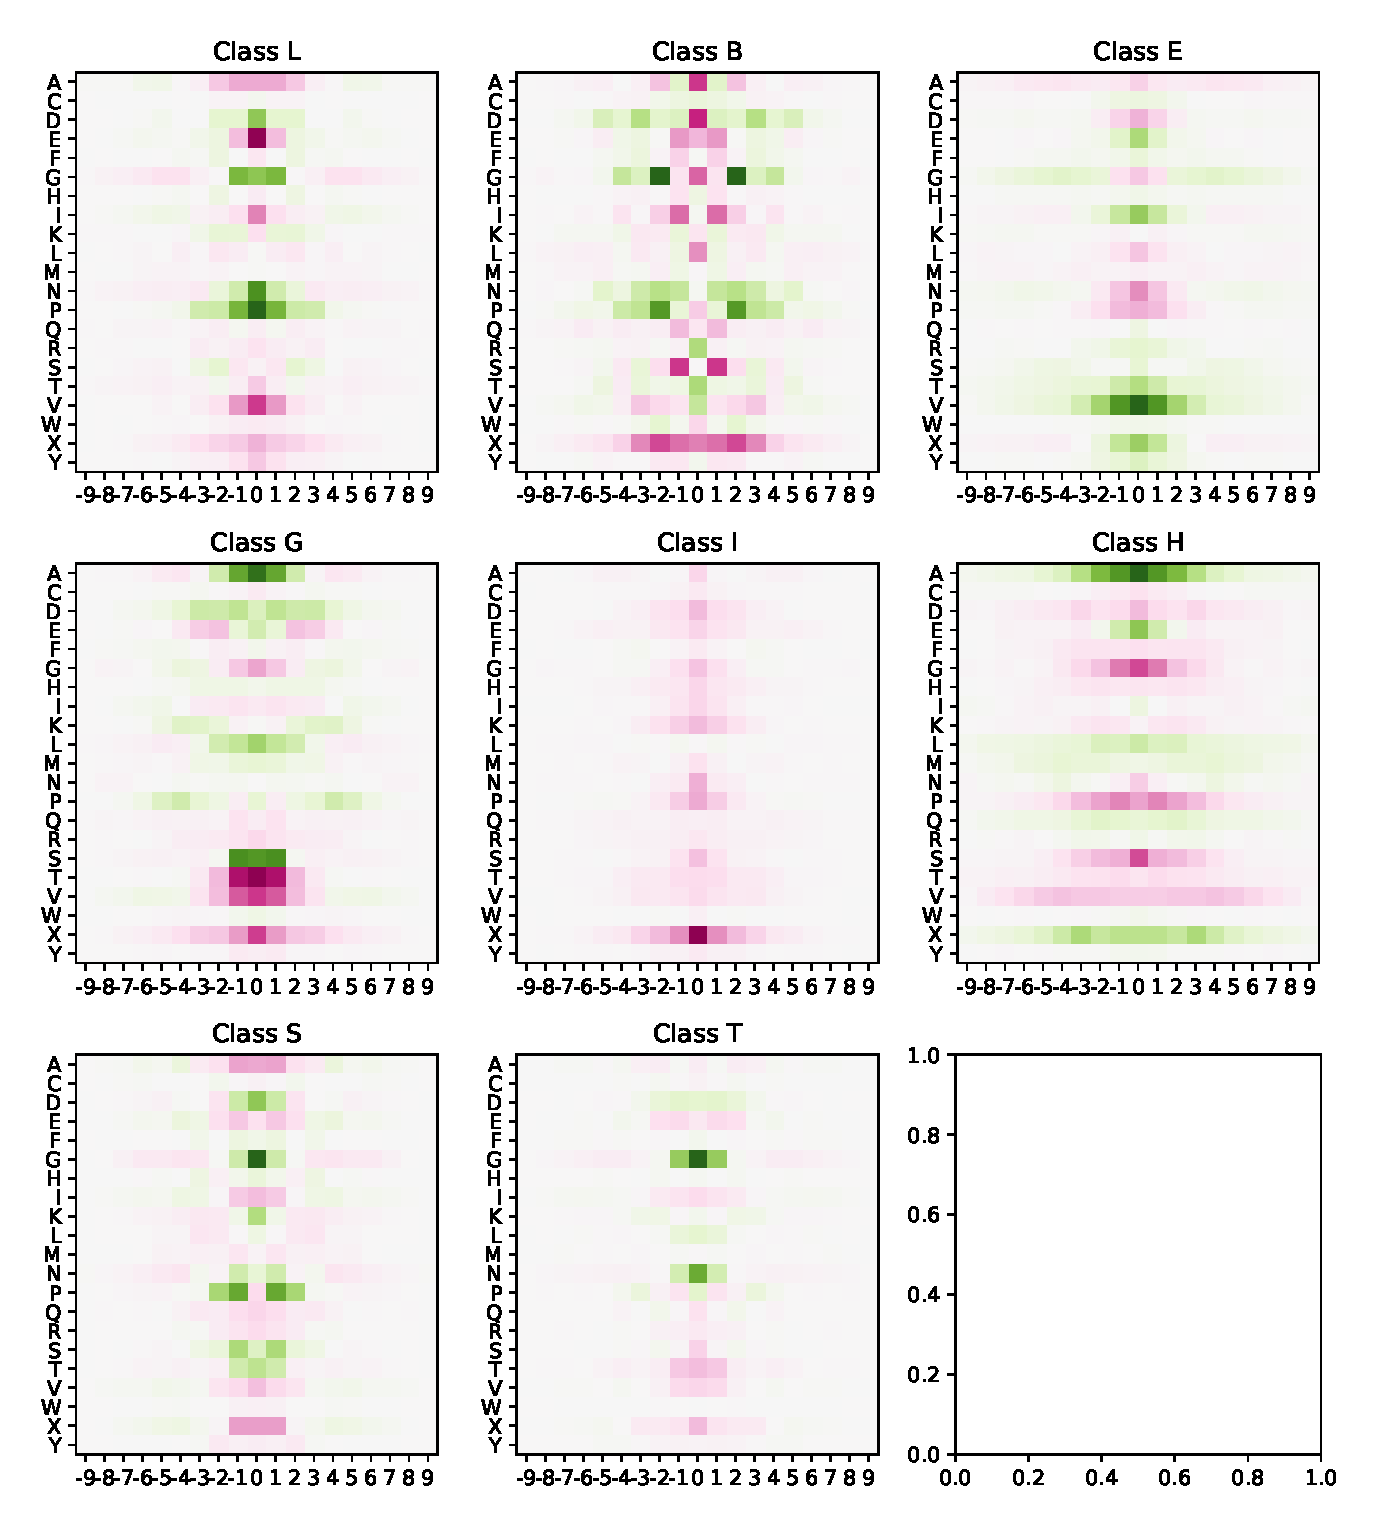
\includegraphics[width=0.85\linewidth]{Figures/class_agg_class_all}
\caption{\textit{Per-class aggregated saliency maps along the window of all classes, as discussed in Section \ref{sect:sheer}.} Only the saliency values of \textit{pssm} are shown here. Green means positive saliency values and purple means negative.}
\label{fig:class_agg_class_all}
\end{figure}

\begin{figure}
\centering
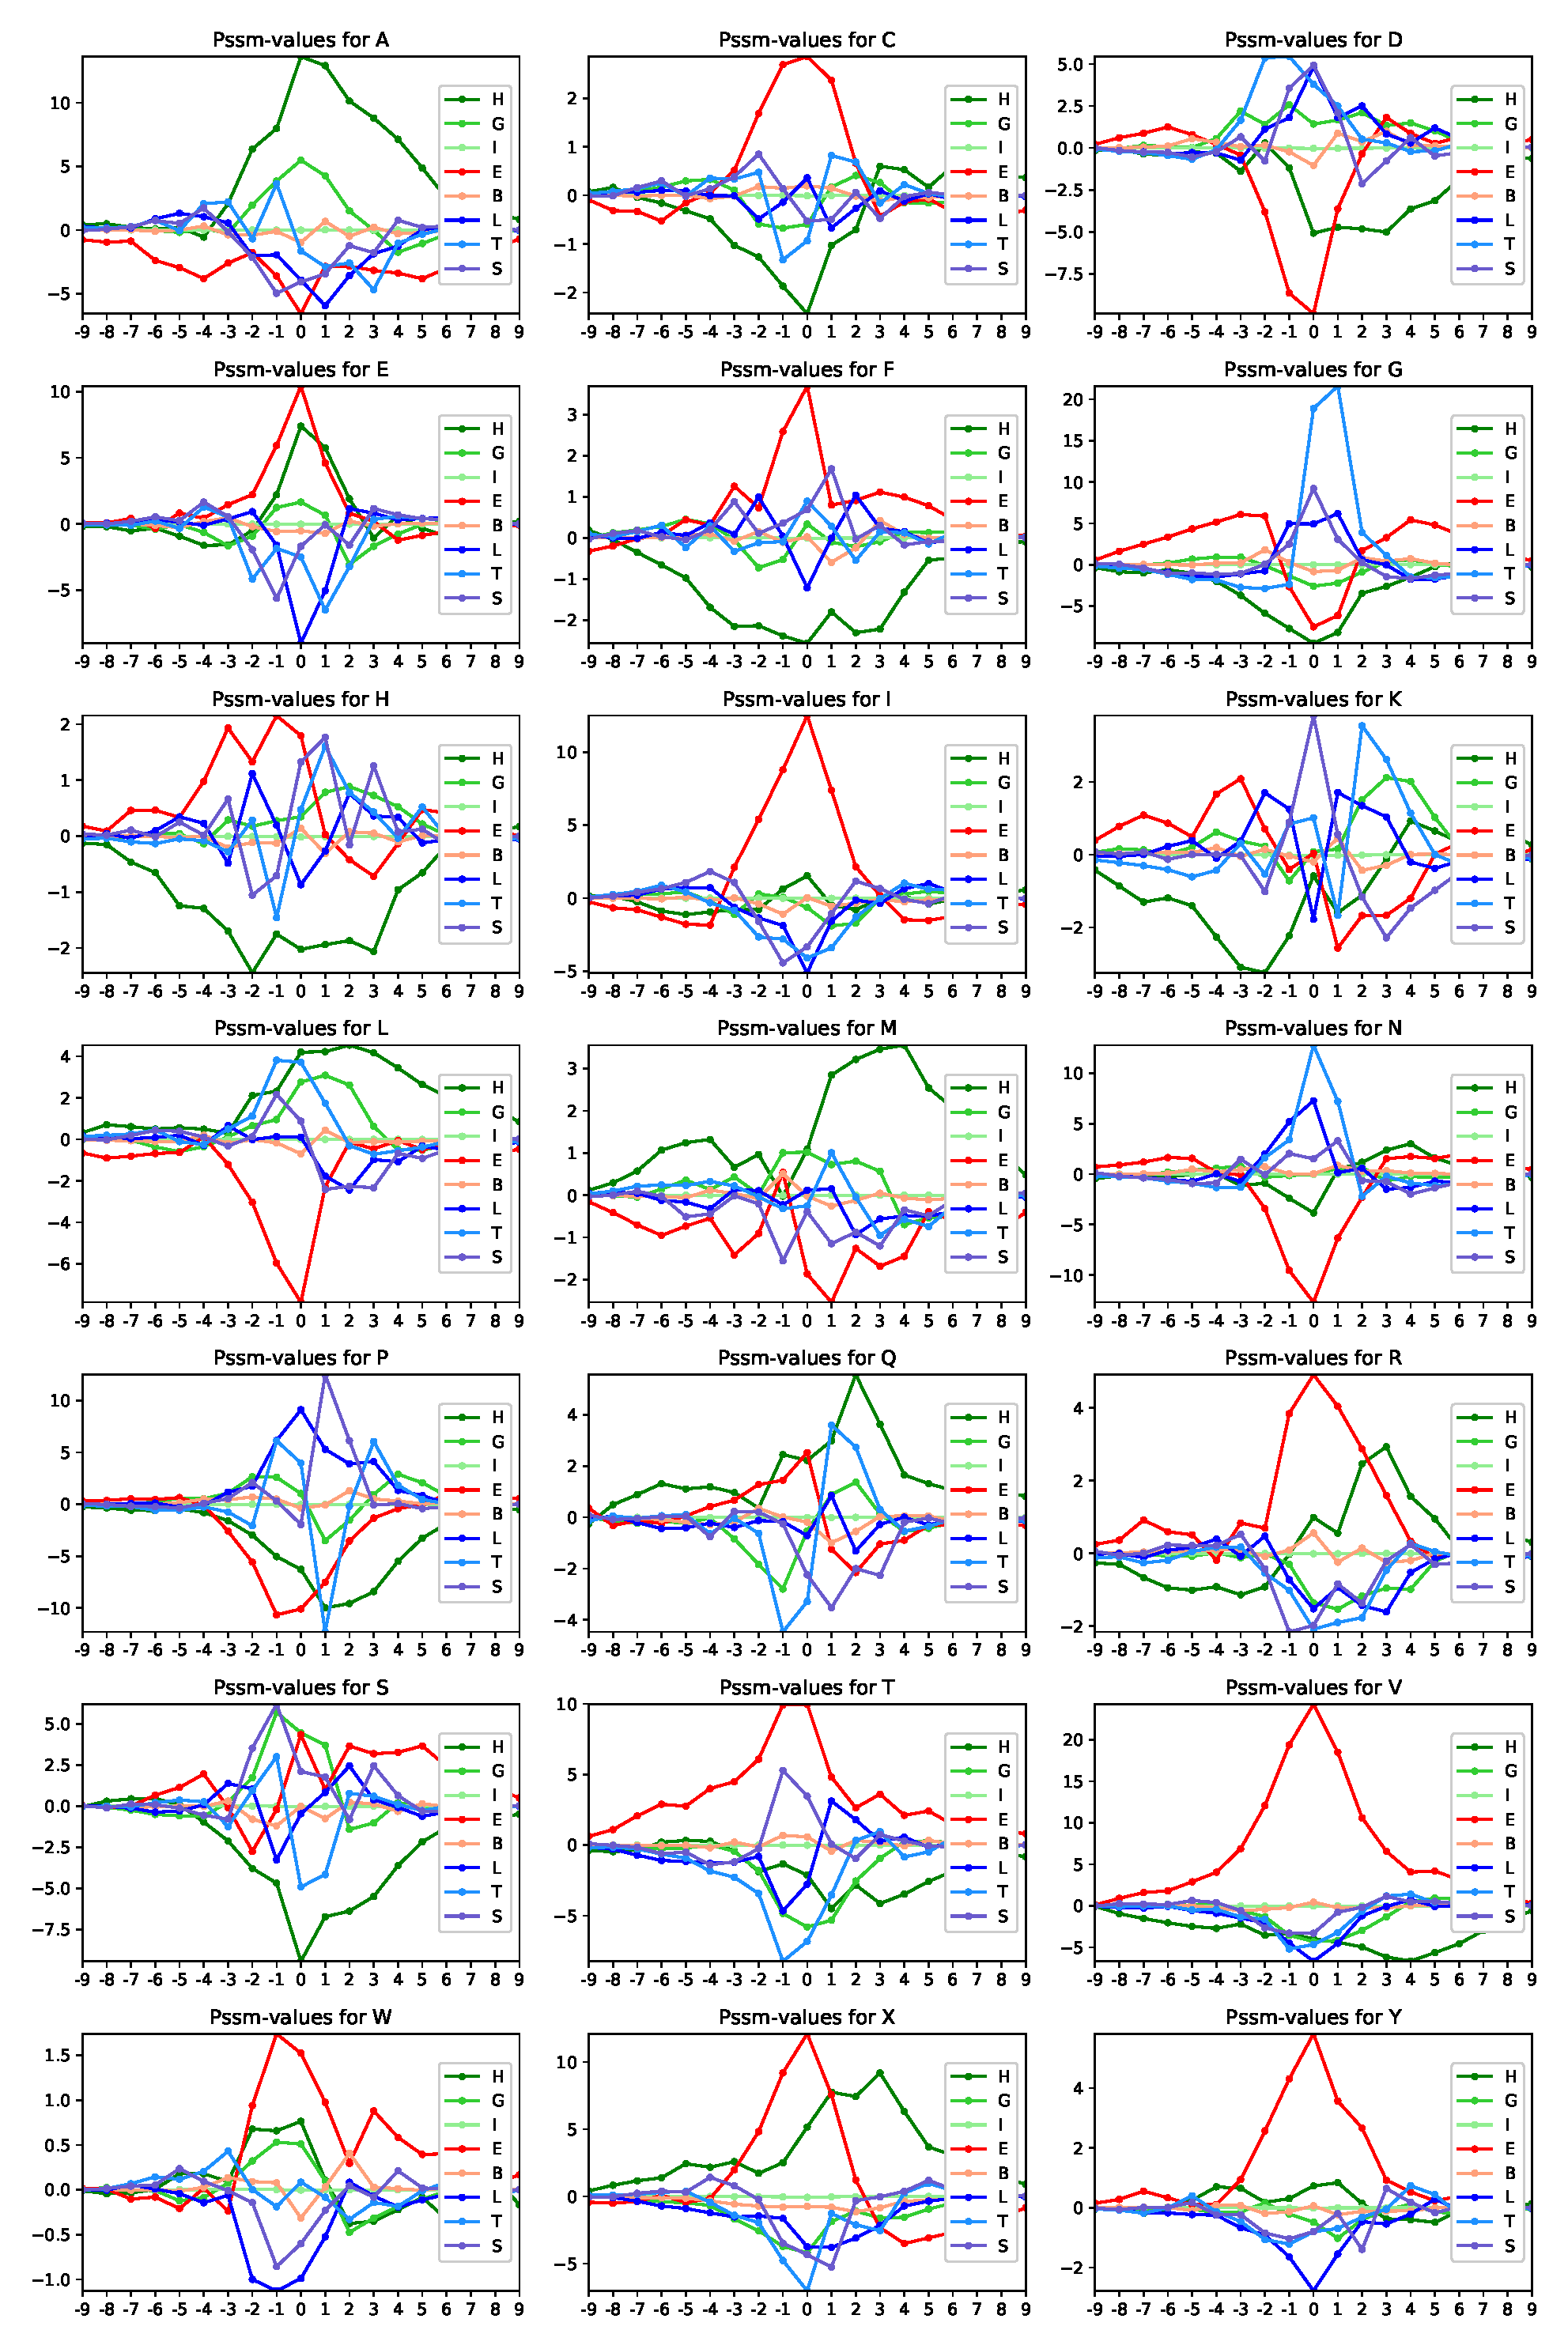
\includegraphics[width=1\linewidth]{Figures/class_agg_aa_all}
\caption{\textit{Per-class aggregated saliency map of all 21 amino-acids.} \textit{Y} axis is in 1000s. Note the changes in scale.}
\label{fig:class_agg_aa_all}
\end{figure}
